\chapter{Oscillator phase noise}


\section{Simplification of an integral}
Define the integral
\begin{equation}
  I(\tau, \tau_j)
  \equiv
  \int_{a}^{a + \tau_j} dx
  \int_{a + \tau}^{a + \tau + \tau_j} dy \,
  f(x - y),
\end{equation}
where $a$, $\tau$, and $\tau_j$ are real.
Make the change of variables
\begin{equation}
  x = z + y,
  \label{eq:OscillatorPhaseNoise:change_of_variables}
\end{equation}
which transforms the integration domain as shown in
Fig.~\ref{fig:OscillatorPhaseNoise:integration_domains}.
Then, $I(\tau, \tau_j)$ becomes
\begin{align}
  I(\tau, \tau_j)
  &=
  \int_{- \tau_j - \tau}^{- \tau} dz \, f(z)
  \int_{a - z}^{a + \tau + \tau_j} dy
  +
  \int_{-\tau}^{\tau_j - \tau} dz \, f(z)
  \int_{a + \tau}^{a + \tau_j - z} dy
  \notag \\
  &=
  \int_{- \tau_j - \tau}^{- \tau} dz \,
  \left[ \tau_j + (z + \tau) \right]
  f(z)
  +
  \int_{-\tau}^{\tau_j - \tau} dz \,
  \left[ \tau_j - (z + \tau) \right]
  f(z)
  \notag \\
  &=
  \int_{-\tau_j}^{0} dz' \,
  \left[ \tau_j + z' \right]
  f(z' - \tau)
  +
  \int_{0}^{\tau_j} dz' \,
  \left[ \tau_j - z' \right]
  f(z' - \tau)
  \notag \\
  &=
  \int_{-\tau_j}^{\tau_j} dz' \,
  \left[ \tau_j - |z'| \right]
  f(z' - \tau)
\end{align}

\begin{figure}
  \centering
  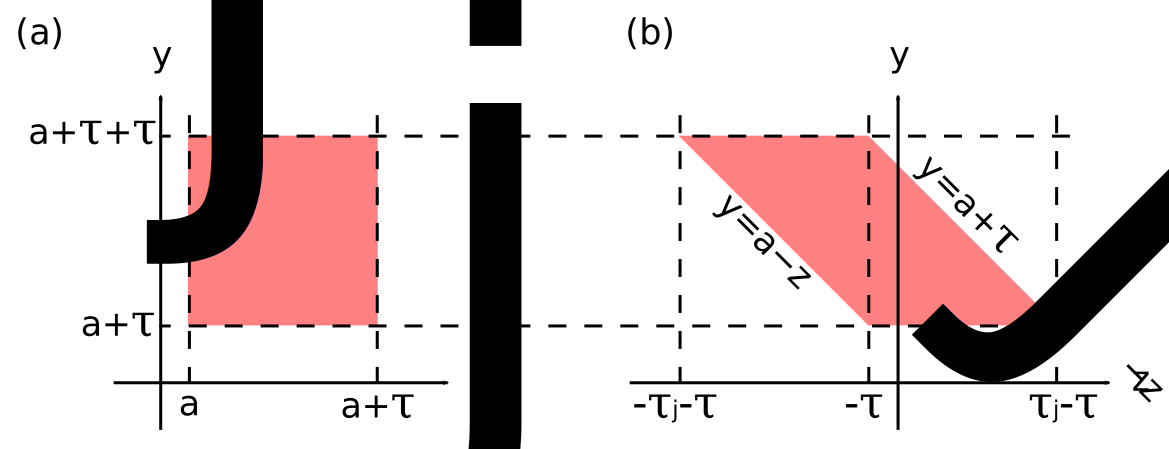
\includegraphics[width = \textwidth]{%
    Appendices/OscillatorPhaseNoise/figs/integration_domains.pdf}
  \caption[Integration domains]{
    Integration domains (a) before and (b) after
    the change of variables in
    (\ref{eq:OscillatorPhaseNoise:change_of_variables}).}
  \label{fig:OscillatorPhaseNoise:integration_domains}
\end{figure}
